% !TEX root = CSC104LectureNotes.tex

% \setcounter{chapter}{11}
\chapter{Python Errors and zyLabs}

\topquote{Syntax, my lad. It has been restored to the highest place in the republic.}{John Steinbeck}

\minitoc

\section{Python Errors}
\label{sec:errors}

If you are an athlete, or a performer, or a writer, or a pursuer of any other creative enterprise, you already know that part of the exhiliration of performing is the danger that something won't go the way you expect.  Programming a computer is no different.  Finding an error in a computer program is a common occurrence.  It has been nearly seventy years since a Major League Baseball player has successfully gotten a hit more than 40\% of the time in one season.  Baseball players don't look at outs as failures; they view them as opportunities to learn and improve.  You must be prepared to do the same if you are going to be a successful programmer.

\subsection{Syntax Errors}

\begin{myfigure}[float,label=fig:syntax-error]{Syntax Error: Calling a Function Without Parentheses}
    \centering
    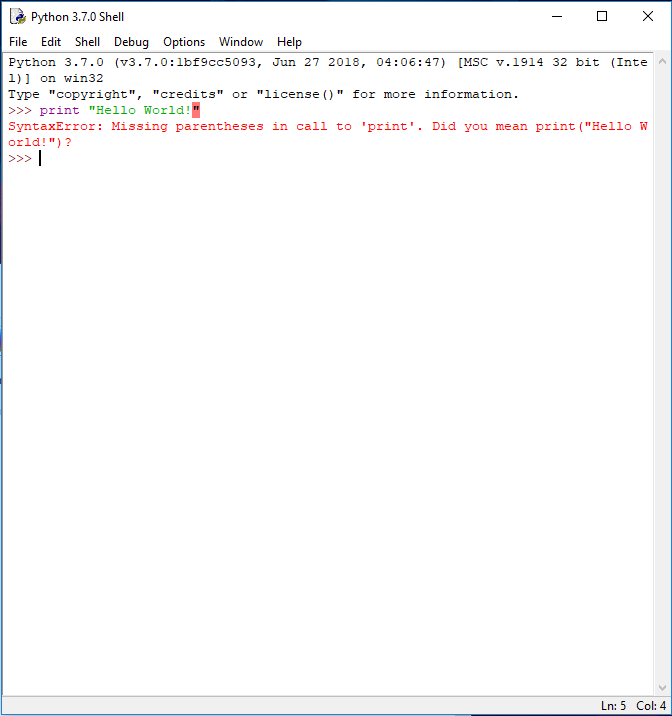
\includegraphics[scale=0.825]{screenshots/syntax-error}
\end{myfigure}

As you learned in Section 1.4 of zyBooks, and as we discussed way back on Day \ref{day:vocabulary} (see Section \ref{sec:kindsoferrors} in these notes), there are a couple of different kinds of errors we programmers can make.  The first kind of error is a \addindex{Error!Syntax error}{syntax error}.  As we learned then, a syntax error comes from writing an instruction that does not conform to the language's rules.

Yesterday, you wrote code that looks like this:

\begin{minted}{python}
print("Hello World!")
\end{minted}

As you now understand, that code is a \textit{call} to the \texttt{print} \textit{function}.  A \textbf{function call} such as this requires the use of parentheses.  If you tried to type this command without the parentheses, you would break the rules of Python's structure, and you would be informed of this immediately, as you see in Figure \ref{fig:syntax-error} on Page \pageref{fig:syntax-error}.

Notice that Python lets you know fairly clearly in red text that your error is a syntax error.  Sometimes (but not always), Python will also include a helpful hint regarding how you can fix this error, as it has in this example.

As you learn about more of Python's features, be sure to pay attention to the syntax that is required to make use of these features.  Like any programming language, Python can be very particular about how we type our code.

\subsection{Runtime Errors}

A \addindex{Error!Runtime error}{runtime error} is caused by a situation that the computer didn't expect.  Since a runtime error occurs when a program runs, such an error can only occur in code that is free of syntax errors.  Runtime errors typically cause the program to immediately terminate.

Consider this Python code that we looked at at the end of Day \ref{day:python1}:

\begin{minted}{python}
my_number = int(input('Type in a number: '))
print(my_number * 3)
\end{minted}

That Python program is free of syntax errors, and will run just fine as long as the user interacts with it in an expected way.  However, if you run the program and type \texttt{Idaho} instead of a number, the \mintinline{python}{int()} function won't be able to complete its job.  Python will respond with this error message:

\begin{tcolorbox}
\ttfamily\small ValueError: invalid literal for int() with base 10: 'Idaho'
\end{tcolorbox}

There are many kinds of runtime errors in Python, and you will not be required to know what they are.  As we write more code, however, you will encounter more errors and of more types, and you will gain experience in finding and fixing them.

\subsection{Semantic Errors}

A \addindex{Error!Semantic error}{semantic error}, or \textit{logic error}, is an error in a program's meaning.  Like runtime errors, these errors only occur in a program that can run (although a good programmer can detect them ahead of time).

Consider this program:
\begin{minted}{python}
age = int(input('How old are you?'))
months = age / 12
print("That's", months, "months!")
\end{minted}

That program will run to copmpletion and provide nice-looking output, which happens to be wrong.  The syntax is fine -- if it weren't, the program would not have run.  There were no runtime errors; the program provided its output and exited normally, with no red error messages.  The problem here is that the programmer provided the wrong instructions.  These kinds of errors are frequently referred to as \textit{bugs}.

\section{zyLabs}

Your instructor will have assigned several interactive programming assignments, to be completed during today's class.  These assignments are called \textbf{zyLabs}, and they're part of the zyBooks online textbook you signed up for.  It is important that you read the instructions for each assignment carefully before starting, and follow them as precisely as you can, to maximize your grade -- and to gain valuable hands-on experience programming in Python!  Remember to have fun, and to ask your instructor for help as soon as you think you need to.  There is no shame in asking for help, especially when trying to do something you have never done before.